\documentclass[12pt]{article}

\title{\vspace{-2.0cm}Stuff}
\title{ST 599 Project 1 Report}
\author{Wanli Zhang \& Matt Edwards}
\date{21st April 2014}

\usepackage{fullpage}
\usepackage{floatrow}
\usepackage{fourier}
\usepackage{parskip}% http://ctan.org/pkg/parskip
\usepackage{graphicx}
\usepackage{caption}
\usepackage{subcaption}

\begin{document}
\begingroup  
  \centering
  \LARGE Master's Report - Draft\\[1em]
  \large Matt Edwards\\
  11 May 2014\par
\endgroup

\section{Introduction}
Transects, both point and line, are a method of population density estimation often used in the ecological sciences. They are useful when populations are too small to be seen from the air (birds, rodents) or may be masked by the canopy (ground plants.) Recent studies that use distance sampling include Norwegian bird populations (Pedersen et al. 2012), Komodo dragon prey estimates (Ariefiandy et al. 2013), Serengeti carnivore abundance (Durant et al. 2011), and estimates for butterfly populations (Isaac et al. 2011). A study by Cox et al. extends point transect sampling for use with underwater acoustics for estimates of krill populations (2011), and a study by Rowcliffe et al. combines distance sampling with camera traps to estimate populations (2011). 

\subsection{History}
\texttt{TO DO}

\subsection{Micronesian Bird Data}
The Micronesian Forest Bird Survey of 1982 (Ramsey, et al.) is a work using Variable Circular Plots (VCPs) placed using a random-systematic transect design to monitor the density of several bird species in the Micronesian islands.

Each island was divided into regions. Initial transects were given random positions and angles, with subsequent transects placed parallel, 2km apart. Stations were placed every 150m along the transects. Two observers, standing 20 m apart, would wait several minutes for the wildlife to quiet down after their arrival, and then spend 8 minutes noting any birds they could observe either visually or aurally. Distance and species were noted, as well as other covariates such as foliage density, weather conditions, etc. 

Figure 1 illustrates the distance data for the Collared Kingfisher. This data represents the aggregated data from two islands, Tinian and Rota, and all four observers. We can observe several things in this plot:

First, there are very low counts of birds immediately around the station, a peak at around 100 m, a fairly level section from 100--200 m, and a drop off after 200 m. This would seem to indicate that the presence of the observers caused either movement away from the station (the crest around 100m) or a suppression of vocalizations and/or movement directly around the station. 

Secondly, note that the detection distances are high between 100--200 m, and recall that the stations were place 150 m apart. Since the stations on a transect were (generally) visited in sequence, this means it is possible a bird was observed from more than one station. 

Lastly, the further away from the station, the distance observations were heaped into categories. With smaller bin widths, this is also evident in the 100--200 m range as well.



\begin{figure}
\caption{Aggregated Collared Kingfisher Observation Distances 1982, Rota \& Tinian}
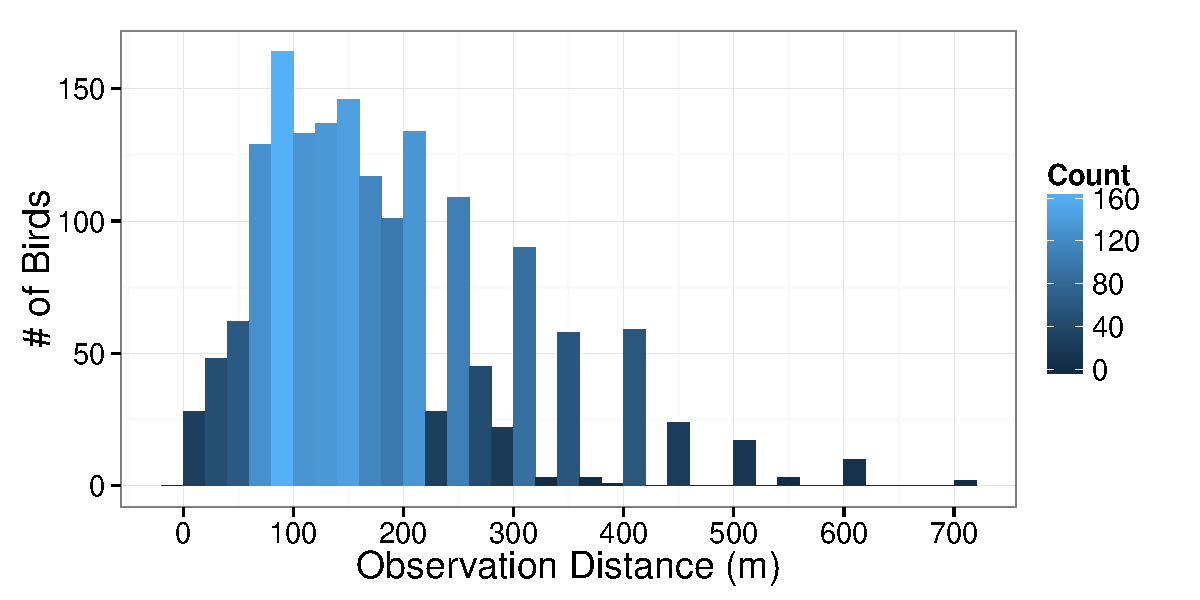
\includegraphics[width=\textwidth]{../images/histogram_distance.pdf}
\end{figure}

\texttt{I don't like the flow here.}
\section{Application}
With Line Transects, a (straight) line is randomly placed in the study area, then walked by the observer, with any objects of interest noted and the distance perpendicular to the transect recorded. With point transects, the observer stands in one spot, recording the direct line distance from herself to the object of interest as if it was projected on the ground. This results in data similar to the line transect, but with more safety for the observer as they do not have to watch for (moving) wildlife and watch where they are walking. (Ramsey, Scott 1979) VCP have the added benefit of allowing the wildlife to settle. Animals may react to an observer moving through the area by hiding or moving away. If the observer is standing still, and has allowed a ``cooling'' period for things to return to normal, animal behavior may be more natural and less influenced by the action of the observer.

Observations of objects can take the form of visual sightings or detection of auditory cues, or one confirmed by the other, as long as an accurate distance can be measured.

\subsection{Notation}
This notation is borrowed from Quang (1993) following Buckland (1987)

\begin{tabular}{r l}
$t$:	&	Number of plots surveyed\\
$D$:	& Common density of animals in all plots\\
$m_j$:	& Number of detected animals in the $j$th plot\\
$\bar m$:	& Average number detected per plot\\
$\mu$:	& Expected number of animals in a plot, $\mu = E(m_j)$\\
$n$:	& Aggregate numbe of animals detected in all plots, $n=\sum_{j=1}^t m_j$\\
$\lambda$:	&	Expected total number of detected animals in all plots, $\lambda=E(n)=t\mu$\\
$R_i$:	& Distance from station to the $i$th detected animal\\
$R_1,\cdots,R_n$: & Detected distances pooled from all plots\\
$s$:	& Sample standard deviation of $R_1,\cdots,R_n$\\
$f(r)$: & Common probability density function (pdf) of the detected distances, $R_1,\cdots,R_n$\\
$h$: 	& Bandwidth used in kernel estimation
\end{tabular}\\

For a typical individual plot:

\begin{tabular}{r l}
$N$:	&	True number of animals in the plot (unknown)\\
$m$:	&	Number of detected animals in the plot\\
$g(r)$:	&	Radial detection function, $g(r)$=Pr(Animal is detected | Animal is at distance $r$)\\
$w$:	&	Distance beyond which no animals can be detected (= radius of the plot)\\
$p$:	& Mean detection probability within the plot\\
$B$:	&   $B = 2/(pw^2)$\\

\end{tabular}

\subsection{Assumptions}
Buckland (2004) lists three primary assumptions:
\begin{enumerate}
\item[i] Objects at the line or point are detected with certainty $g(0)=1$
\item[ii] Objects are detected at their initial location
\item[iii] Measurements are exact
\end{enumerate}

There are additional assumptions listed by both Buckland and Ramsey and Scott (1979) and summarized by Quang (1993):
\begin{enumerate}
\item[iv] Sightings of animals are independent events
\item[v] at least one animal is detected $n > 0$
\item[vi] detectability is the same for all animals at distance r and in all directions.
\item[vii] no animal can be detected beyond a finite distance $w: g(r) = 0$ for $r > w$
\item[viii] the function $g(r)$ has at least 4 bounded derivatives on $[0, w)$, and $g'(0)=0$
\item[ix] the stations are chosen at random in the study area
\end{enumerate}

Ramsey 1979
Uniform distribution, random process distribution, independent distribution, 

Not explicitly stated, is that we are assuming the objects of interest are homogeneously distributed throughout the region being surveyed. REFERENCE

\subsection{Broad Strokes}
In general, an estimate of population density is a count of objects observed divided by the area in which they were observed times the probability of observing the object. (Ramsey, Scott 1979)

Equation 1: $D = E[n]/(A_r)(P_r)$

In practice, the expected value of n is taken to be n, the number of objects observed. The estimation of the denominator is where things get tricky.

If we combine $(A_r)(P_r)$ into an effective area we get:

Equation 2: $A~_R = 2(pi) int?0?R g(y)ydy$

$G(r)$ is the detectability function, and represents the probability of detection at distance $r$. It is often scaled so that $g(0)=1$. (In terms of area of a circle, it is obvious that the $integral{g(y)ydy}$ represents $r^2$ in the $2pi r^2$ equation.)

Much of the uncertainty in VCP estimation comes from how the effective area is estimated. $g(y)$ is often modeled as a parametric class (exponential, half-normal, hazard function) which is then scaled so that $g(0)=1$. In addition to guessing which function to use, we must also estimate the parameters. 

It is plausible to think that as objects are further away from the observer, they are more difficult to detect, and therefore, we would have a greater probability of missing observations that were further away. So, in calculating $g(y)$, do we assume perfect detection out to the furthest point of observation? Or do we truncate our observations at some distance closer to the observer? Ramsey \& Scott (1979) refer to these as the effective radius ($\rho$) and the basal radius ($r$) respectively. 

The problem lies in that in practice, we don't know where the basal radius is, and it must be estimated from our data.

\subsection{Properties}
\subsubsection{Bias \& Consistency}
Buckland et al. (2001) and Ramsey \& Scott (1970) both stated that if our detectability estimate $g(z)=$1 out to $r$, then $D$ is unbiased. 

Barry and Walsh (2001) compared design-based and  model-based estimates of density and variance. (Their focus was line transects, but they state it is analogous to point transects and the conclusions should carry across.) They concluded that model-based estimates were unbiased if and only if the assumptions of objects being independent and uniformly located held. They noted that in practice, this is probably not a feasible assumption. For design-based inference, they caution about both the density and variance estimates.

Roeder, Dennis, \& Garton (1987) use simulations to demonstrate that no method is completely applicable in 100\% of situations, and will go sideways at some point, depending on the specific conditions.

The overall conclusion is that, in theory, density estimates using VCPs are unbiased and (reasonably) consistent, but that the assumptions necessary for the theory to hold are untenable. 

As stated in the section on choosing $g(r)$, it will vary depending on the specific situation, and it is up to the scientist and statistician to understand the data and choose the best approach.

\subsubsection{Independence}
Assumption \texttt{ix}, that the VCPs are placed randomly through the study area, would seem to implicitly state that their observational ranges might by chance overlap, meaning a single object of interest could be observed from more than one station. Thompson (p240) likewise indicates random placement of line transects which would seem to allow for a potential overlap of observation zones. 

Buckland et al (2001) also discuss the random placement of both line and point transects, without addressing the potential for sightings to overlap. Reynolds et al. (1980) state that the possibility of observing the same bird from two stations should be avoided. Buckland (2006) says simulations showed that analysis was robust to violations of independence (meaning overlap, or multiple observations on same object).

On page 233, Buckland et al. (2001) discuss that each line or point must be ``randomly and independently located,'' with ``an equal probability of selection'' for all portions of the study area.

On page 235, Buckland et al. states ``Transects are normally spaced at a sufficient distance to avoid detecting an object from two neighboring transacts, although this is not usually critical unless sampling a line changes the animal distribution at neighboring, as yet unsampled lines.''

They do state that for random-systematic transects, the methodology used by Ramesy et al (1982), that each transect line should be treated and analyzed as a cluster.

Barry and Welsh (2001) in discussing line transects, treat it as a two-stage sample, with non-unique clusters (each study object can be in more than one cluster) having an equal probability of selection. This would seem to (but does not explicitly) endorse the possibility of overlapping VCPs. 

One of the assumptions of distance sampling is that the objects being studied are distributed homogeneously throughout the space [reference].  (If the data is clustered we have other problems, not addressed here.) If that is the case, then it would make sense thought-level idea that it shouldn't matter if the observations overlap, as long as the act of observing at one station does not affect the observations at the neighboring station. This echoes Buckland’s statement a few paragraphs previous.

Thomson mentions (page 244) that the systematic selection of transects (random position of first, with additional transects a fixed distance apart) does not affect the approximate unbiasedness of the density estimator, but will have an effect on the approximate unbiasedness of the variance estimator. 

\section{Simulation}
As seen in the previous section, the issue of independence of the point transects does not have a consensus in the literature. If independence is required for proper estimation, then the random-systematic placement method should not be used. 

Through simulation, we can explore what happens under three different VCP placement schemes, and compare the resulting density estimates to their known values to evaluate performance.

\subsection{VCP Arrangement}
Simulation will address three options for VCP arrangement:
\begin{itemize}
\item Structured: VCPs placed so that observation distances do not overlap
\item Random: VCPs placed completely at random
\item Random-Systematic: Two transects of 18 stations each, placed according to Ramsey et al's design: 150 m between stations, 2 km distance between parallel transects.
\end{itemize}

Figures 2 and 3 illustrate the first two arrangements. Density in these images is based on the 20 birds per km$^2$ of the Palie region on Rota. The surveyed area of the Palie region totaled 9.41 km$^2$ during the original survey, and contained two transects of 16 and 17 stations each, 33 stations total (Ramsey et al 1982).

As seen in Figure 1, there is very little detection happening beyond 500 m. There are 15 observations beyond 500 m, which is 0.9\% of the data. 

Treating 500 m as our truncation distance $w$, the study area in the simulation has been raised to 36 km$^2$ to allow for stations where the observation area did not overlap. An area of 49 km$^2$ is generated with the given density, then truncated to 36 km$^2$ to prevent any edge effect from the random generation of points. The stations are placed a minimum of 500 km (0.5 on the graph) away from the edges to prevent border truncation. 

For the random-systematic, an angle was chosen between $0$ and $\pi$. A transect of 18 stations 150 m apart was constructed, and a second transect of 18 stations constructed running parallel. The transects were then randomly placed with in the graph, no closer to the edge than 500 km (0.5 on graph.) Figures 4 and 5 are two examples.

\begin{figure}
	\centering
	\caption{VCP Layout options. On graph, 1 unit = 1 km. Circles represent 200 m mark.}
	\begin{subfigure}[b]{0.45\textwidth}
		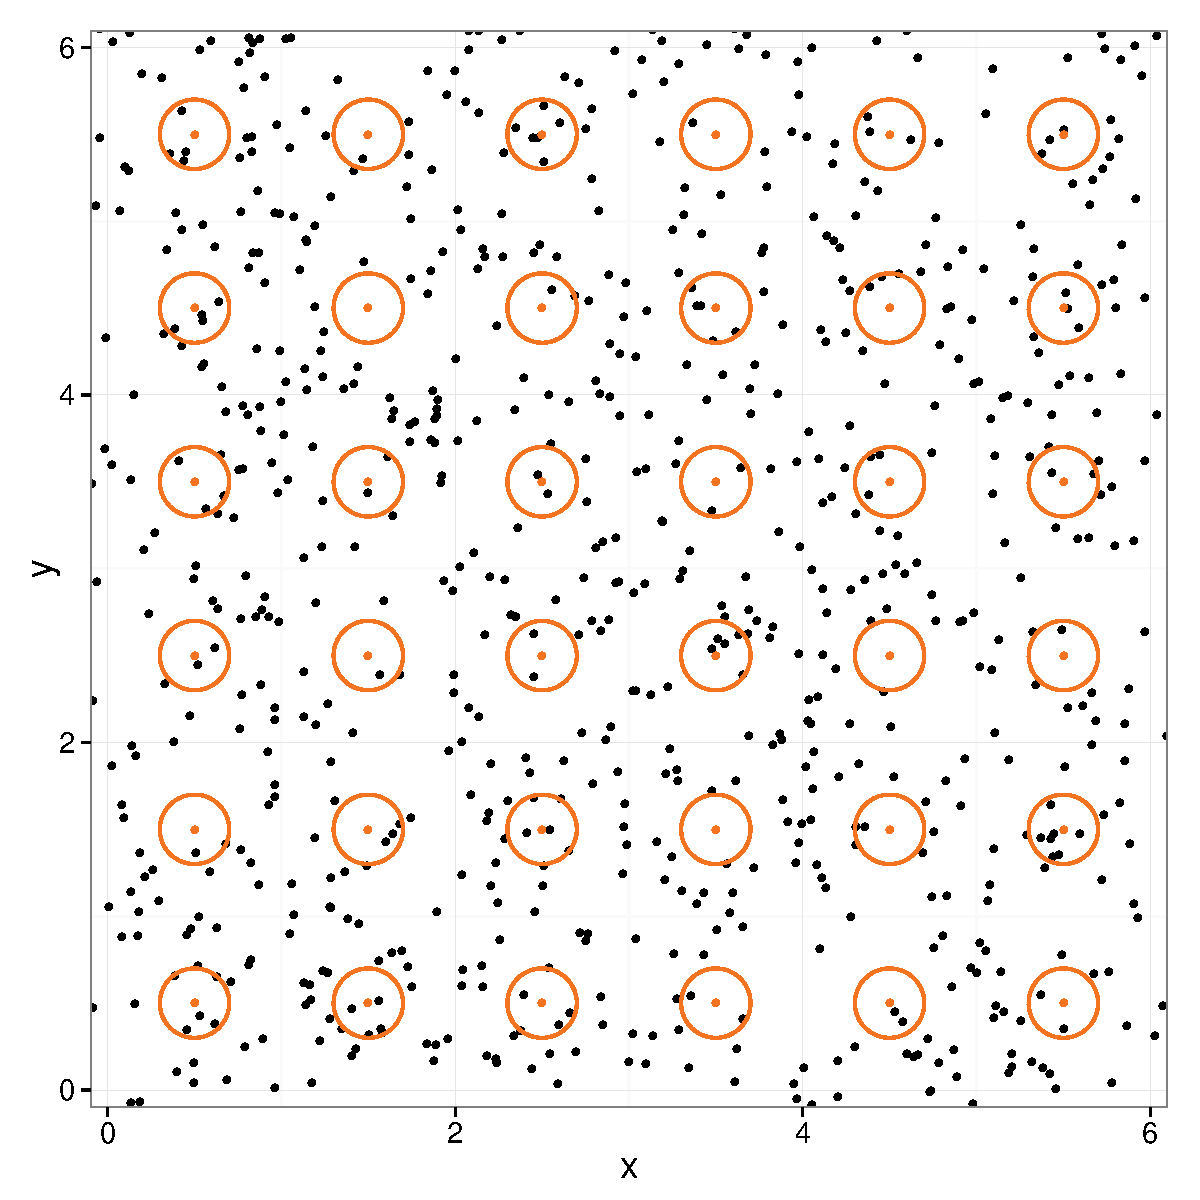
\includegraphics[width=\textwidth]{../images/layout_structured.pdf}
		\caption{Structured Layout}
		\label{fig:structured}
	\end{subfigure}
	\begin{subfigure}[b]{0.45\textwidth}
		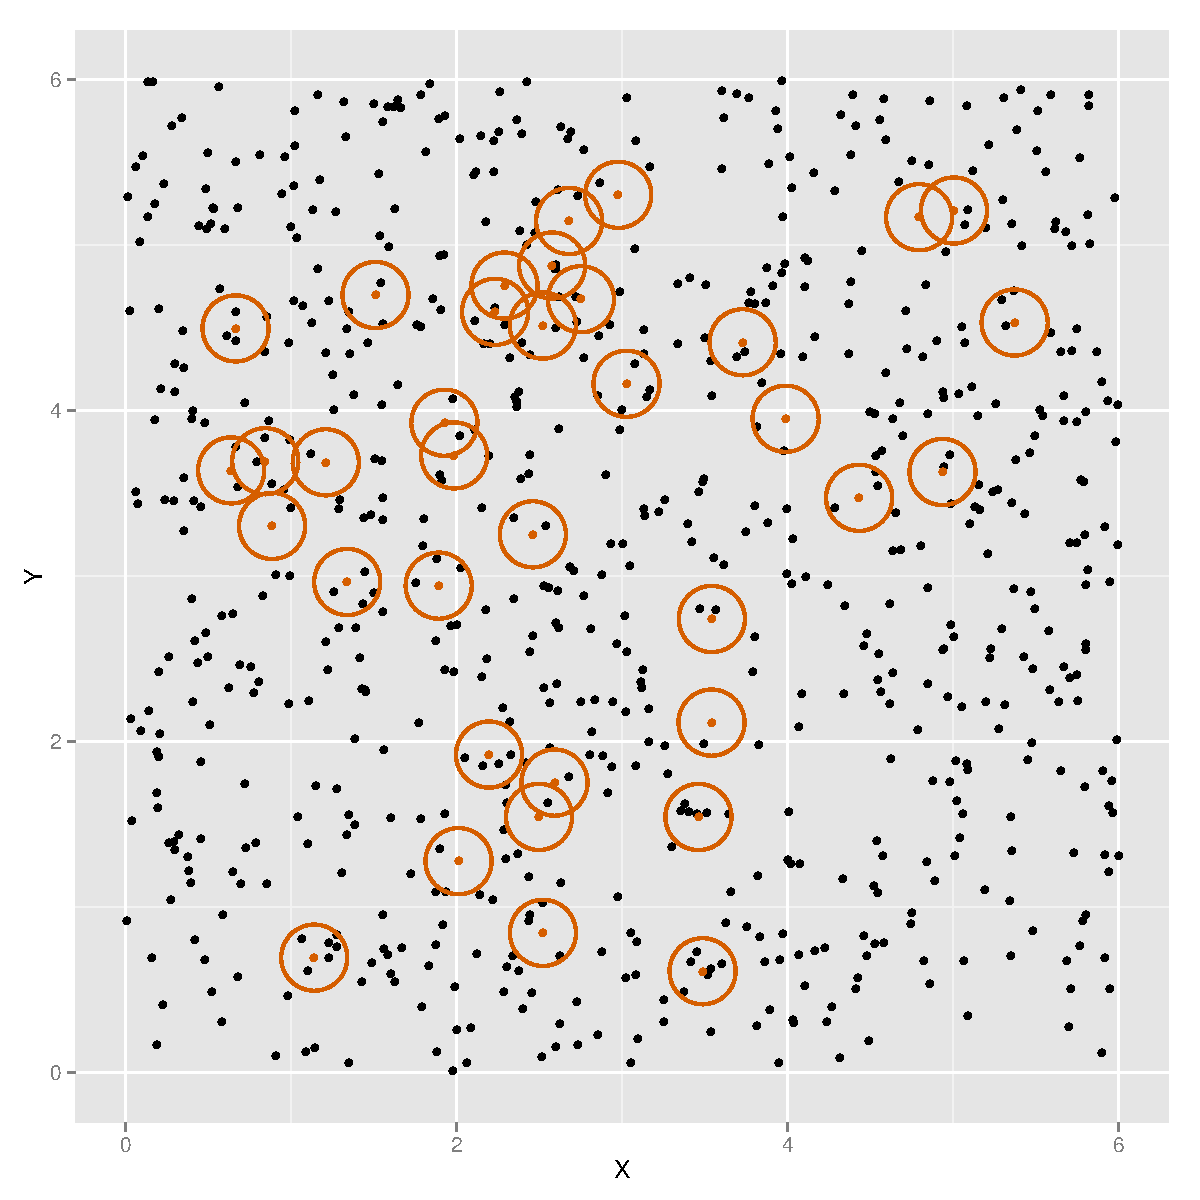
\includegraphics[width=\textwidth]{../images/layout_random.pdf}
		\caption{Totally Random Layout}
		\label{fig:structured}
	\end{subfigure}
	
	\begin{subfigure}[b]{0.45\textwidth}
		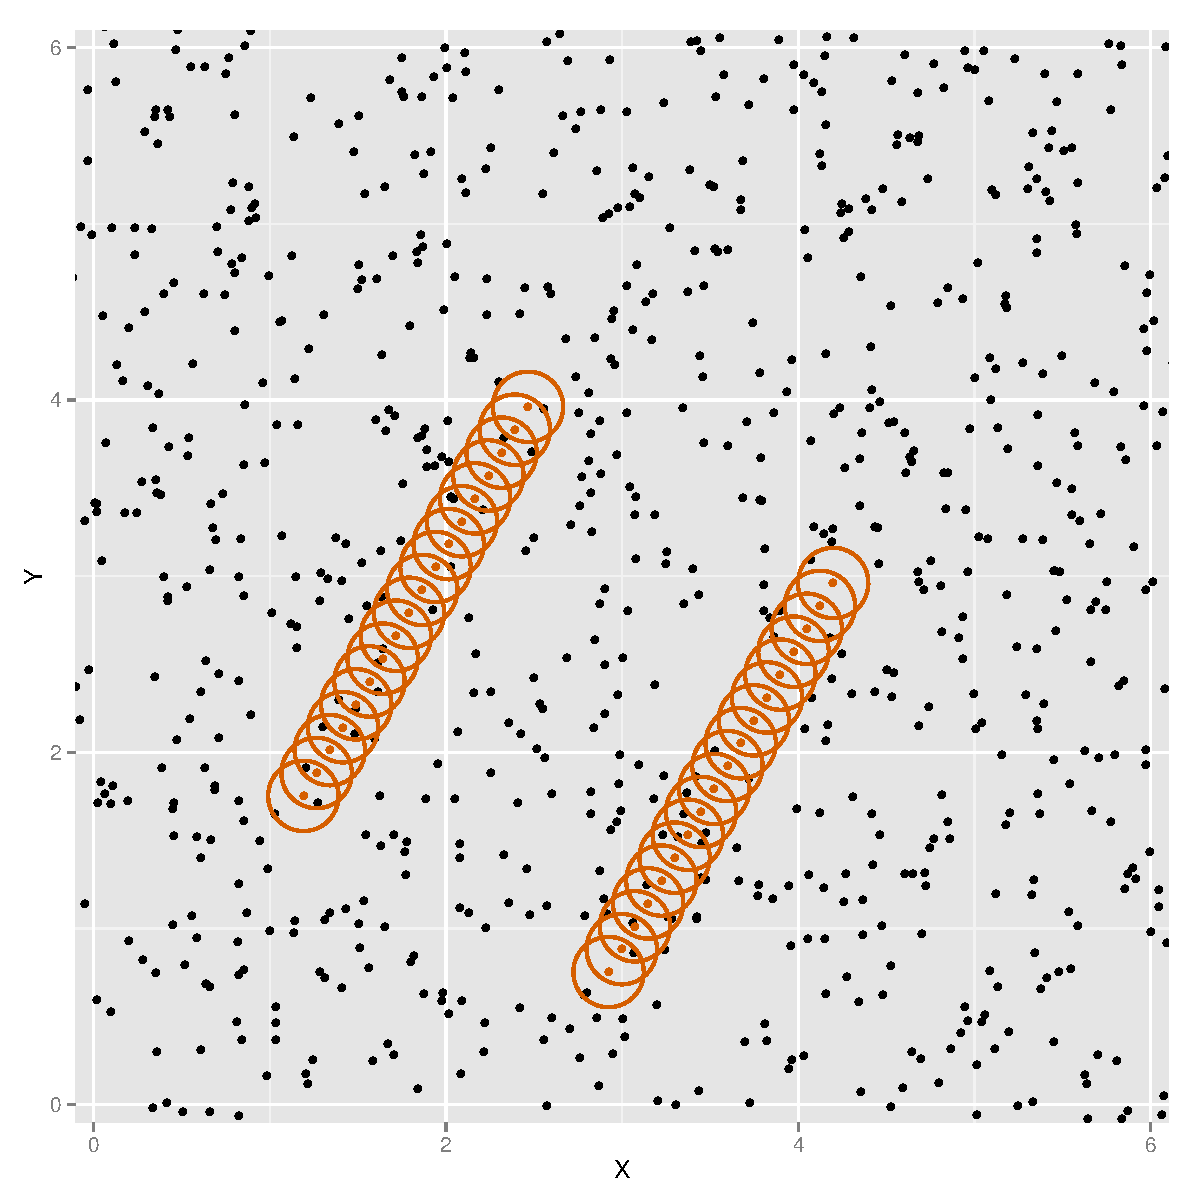
\includegraphics[width=\textwidth]{../images/layout_rand-sys-4.pdf}
		\caption{A Random-Systematic Layout}
		\label{fig:structured}
	\end{subfigure}
	\begin{subfigure}[b]{0.45\textwidth}
		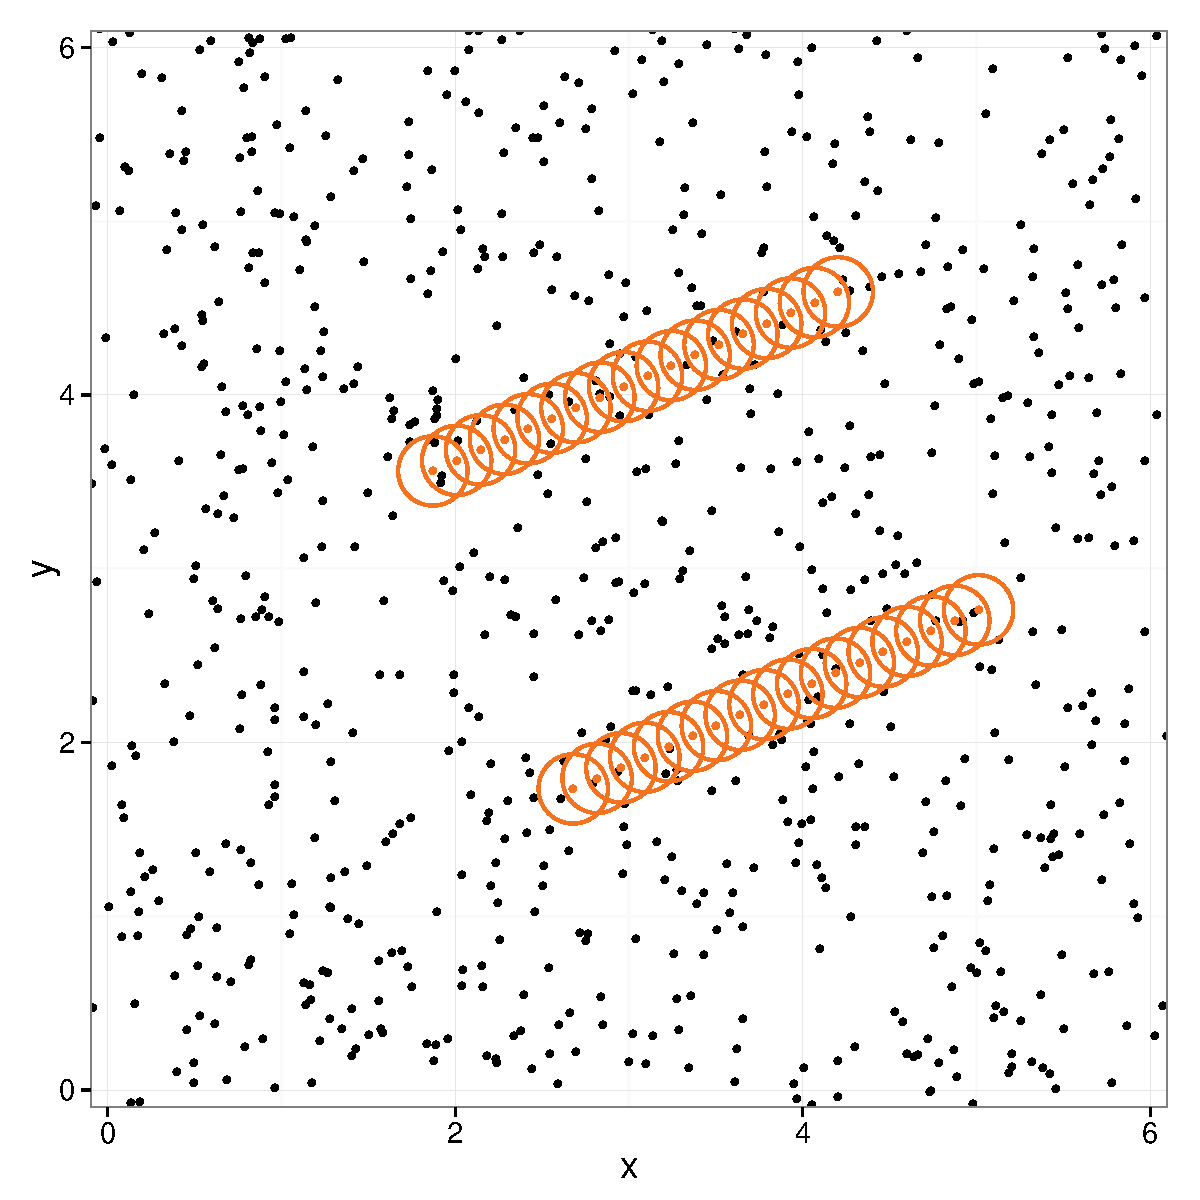
\includegraphics[width=\textwidth]{../images/layout_rand-sys-6.pdf}
		\caption{Another Random-Systematic Layout}
		\label{fig:structured}
	\end{subfigure}
\end{figure}

\section{Simulation Setup}
\subsection{$g(0)$}
\subsubsection{Half Normal}
For a maximum possible observation distance of 0.500 (500 m), the parameter for the half-normal detection function is $\theta = 8.77$, with a scale parameter $\delta = 0.179$.

The half-normal parameter $\theta$ is related to the standard deviation of a standard normal distribution by the relationship:

$\theta = \frac{\sqrt{\pi /2}}{\sigma}$

If we estimate $\sigma$ by $w/3.5$ (with $w$ being the maximum distance at which we might observe an object, and 3.5 being the standard deviation point where P(X > 3.5) < 0.001) then theta is:

$\sigma = w/3.5 = 0.1429$

$\theta = \frac{\sqrt{\pi /2}}{0.1429}=8.7732$

For a half-normal with parameter $\theta=8.7732$, $f(0)=5.5852$ so to scale the value to 1:

$\delta_{HN} = 1/5.5852 = 0.1790$

\subsubsection{Empirical Observations}
\begin{figure}

	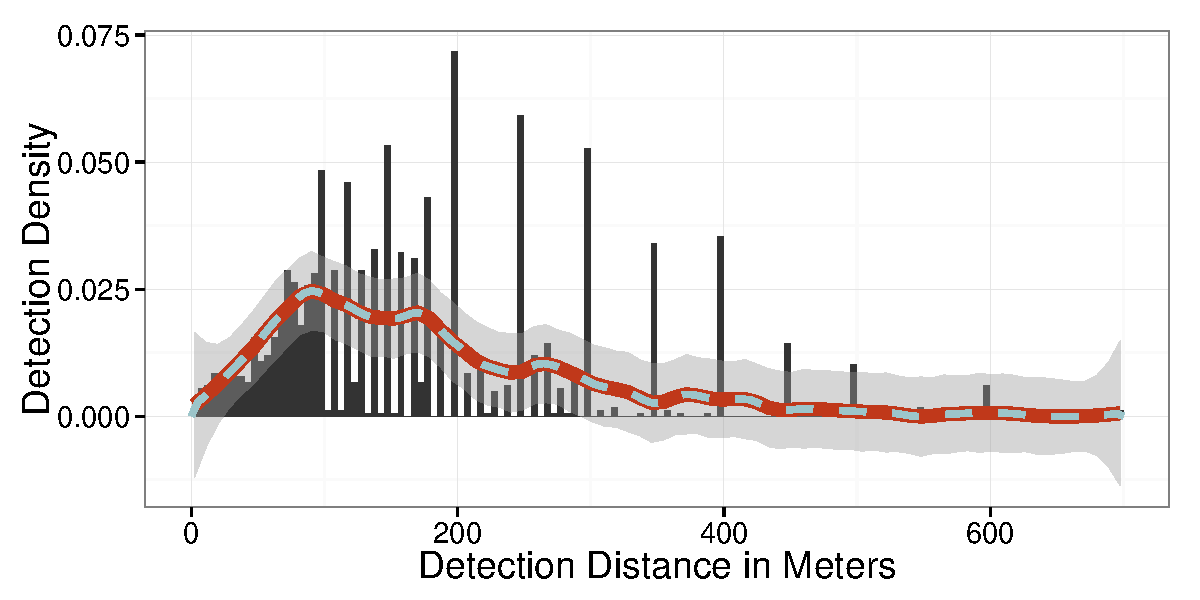
\includegraphics[width=\textwidth]{../images/loess.pdf}
	\caption{Empirical Observation Distances from Original data in meters, with LOESS regression lines. Bin width=5 m\label{fig:by5}}
		
\end{figure}

We can see in Figure \ref{fig:by5} that above 100 m, observations were commonly heaped into 10 or 25 m distances, with the latter being more heavily used. Above 200 m, 50 m heaps were common. To estimate a density function, I used a loess regression with a span of 0.2 on the counts from 5 meter bins of the empirical data. This is the blue line in Figure \ref{fig:by5}. 

Using the \texttt{hist()} function in R, the 1982 observation distances were broken into counts by 5 m groups. Using the bin midpoints, the density estimate was multiplied by 5 to get the density value for that bin. A LOESS regression was run with the midpoint as $x$ and $y=density*5$, using the \texttt{loess()} package in R.

This gives us an object that can be used with \texttt{predict()} to get density estimates for specific distances. The values generated by feeding our midpoints into our prediction function are represented by the red dashed line in Figure \ref{fig:by5}. 

Following the scaling of the highest point to 1, as was done with the half normal curve, where the highest point was $g(0)$, we also find $\delta$ for this empirical detection probability. A sequence of $x$ values was generated covering the range from 0--500 m. This was plugged into the \texttt{predict()} function using our LOESS object. The highest density value was then scaled to be 1:

$\delta_{EMP}=\frac{1}{max(predicted)}=40.5780$ 


\end{document}